\documentclass[11pt,answers]{exam}
\usepackage[margin=0.5in]{geometry}
\usepackage{amsmath,amssymb}
\usepackage{tikz}
\usepackage{soul}

\newcommand{\ds}{\displaystyle}

\begin{document}
\pagestyle{empty}

\subsection*{Numerical Analysis - Math 342 \hfill Midterm 1 Review}

\textit{The following problems are similar to ones you might see on the midterm exam.}

\begin{questions}

\question Use Newton's method to write down an iterative formula for finding the root of $f(x) = x^3-a$ for any constant $a$.  If you start with the initial guess $x_0 = \frac{1}{3}a$, then what is $x_1$?    

\begin{solution}
The Newton's method iteration formula is 
$$x_{n+1} = x_n - \frac{f(x_n)}{f'(x_n)}.$$
In this case, $f(x) = x^3 - a$ and $f'(x) = 3x^2$, so
$$x_{n+1} = x_n - \frac{x_n^3 - a}{3x_n^2}.$$
When $x_0 = \tfrac{1}{3}a$, 
$$x_1 = \tfrac{1}{3}a - \frac{(\tfrac{1}{3}a)^3 - a}{3(\frac{1}{3}a)^2} = \frac{2}{9}a - \frac{3}{a}.$$
\end{solution}
\vfill

\question The root of $x^3-2$ is $\sqrt[3]{2}$, which is located in the interval $[1,2]$.  If we use the bisection method to find this root, starting with the endpoints $a=1$ and $b=2$, then what is the worst case error in our estimate for the root after 10 steps?  
\begin{solution}
Each step in the bisection method reduces the error by a factor of 2.  Initially the solution could be anywhere in the interval $[1,2]$, so our initial error could be as big as 1 (since 1 is the length of the interval).  After 10 steps, the worst case error would be 
$$\frac{1}{2^{10}} = \frac{1}{1024}.$$  
\end{solution}
\vfill


\question Find values for the constants $M$ and $L$ such that $|f''(x)| \le M$ and $|f'(x)| \ge L$ when $f(x) = x^3-2$ on the interval $[1,2]$.  

\begin{solution}
Here $f'(x) = 3x^2$ and $f''(x) = 6x$.  On the interval $[1,2]$, both functions are always positive, so we can ignore the absolute values.  Then the lower bound $L$ for $f'(x)$ is $3$ and the upper bound $M$ for $f''(x)$ is 12.  
\end{solution}
\vfill

\question Based on your constants from the previous problem, and the Newton's method error formula 
$$|x_{n+1} - r| \le \left( \frac{M}{2L} \right) |x_n - r|^2,$$
how close to the root $r$ would a guess $x_n$ in $[1,2]$ need to be in order to guarantee that the next iterate $x_{n+1}$ is definitely closer to $r$?  
\begin{solution}
As long as $\left( \dfrac{M}{2L} \right) |x_n - r| < 1$, then $|x_{n+1} - r|$ will be smaller than $|x_n - r|$.  In this case, $\dfrac{M}{2L} = 2$, so we need $|x_0-r| < \frac{1}{2}$. %Any guess $x_0 \in [1,2]$ that has a distance away from the root of less than $\tfrac{1}{2}$ will produce a sequence of Newton's method iterates that converges to $r$. 
\end{solution}
\vfill

\question Use the triangle inequality to find an upper bound $M$ for $|f'(x)|$ when $f(x) = \sin 2x + \cos 3x$. 
\begin{solution}
Since $f'(x) = 2 \cos 2x - 3 \sin 3x$, we have 
$$|f'(x)| = | 2 \cos 2x - 3 \sin 3x | \le 2 | \cos 2x | + 3 |\sin 3x| \le 5.$$
So $M = 5$ is an upper bound.
\end{solution}
\vfill

\question Find the fixed points of the function $f(x) = \dfrac{8}{3x-2}$.  
\begin{solution}
A fixed point is an $x$-value such that $f(x) = x$.  So we have to solve $x = \dfrac{8}{3x-2}$.  This becomes $3x^2 - 2x - 8 = 0$ and you can get the solutions using the quadratic formula
$$x = \frac{2 \pm \sqrt{4 + 96}}{6} = 2, -\frac{4}{3}.$$
\end{solution}
\vfill

\question What is the derivative of the function $f(x) = \dfrac{8}{3x-2}$ at each fixed point?  Based on the derivative, determine whether each fixed point is attracting or repelling (or not enough information).  

\begin{solution}
You can use the quotient rule or the chain rule to find the derivative of $f(x)$.  Using the chain rule, we get:
$$\frac{d}{dx} \dfrac{8}{3x-2} = \frac{d}{dx} 8 (3x-2)^{-1} = -8 (3x-2)^{-2} \cdot 3 = -\frac{24}{(3x-2)^2}.$$
When $x=2$, this becomes
$$f'(2) = -\frac{24}{(4)^2} = -\frac{3}{2}.$$
Since $|f'(2)| > 1$, the fixed point $x=2$ is repelling.
When $x=-\frac{4}{3}$, we get
$$f'(-\frac{4}{3}) = -\frac{24}{(-6)^2} = -\frac{2}{3}.$$
Since $|f'(-\frac{4}{3})| < 1$, the fixed point $x=-\frac{4}{3}$ is attracting. 
\end{solution}
\vfill

\newpage
\question Let $A = \begin{pmatrix} 1 & 2 & 4 \\ 5 & 7 & 21 \\ 1 & 11 & 1 \end{pmatrix}.$
\begin{parts}
\part Find the LU-decomposition of $A$.  
\begin{solution}
The LU-decomposition without partial pivoting is:
$$L = \begin{pmatrix} 1 & 0 & 0 \\ 5 & 1 & 0 \\ 1 & -3 & 1\end{pmatrix} ~~~~ U = \begin{pmatrix} 1 & 2 & 4 \\ 0 & -3 & 1 \\ 0 & 0 & 0 \end{pmatrix}.$$
\end{solution}
\vfill


\part What is the rank of $A$? Is $A$ invertible?
\begin{solution}
The echelon form $U$ has 2 pivots, so the rank is 2. $A$ is not invertible because its rank is not 3. 
\end{solution}
\vfill

\part Compute $\|A\|_\infty$.
\begin{solution}
The induced infinity norm of $A$ is the maximum $1$-norm of its rows. So $\|A\|_\infty = 33$. 
\end{solution}
\vfill


\part Use the LU-decomposition to solve $Ax = \begin{pmatrix} 2 \\ 11 \\ -1 \end{pmatrix}$. 
\begin{solution}
To solve $Ax = b$, we first solve $Ly = b$ and then solve $Ux = y$.  So first:
$$\begin{pmatrix} 1 & 0 & 0 \\ 5 & 1 & 0 \\ 1 & -3 & 1\end{pmatrix} \begin{pmatrix} y_1 \\ y_2 \\ y_3 \end{pmatrix} = \begin{pmatrix} 2 \\ 11 \\ -1 \end{pmatrix}$$
which is the same as the system of equations:
$$y_1 = 2$$
$$5y_1+y_2 = 11 \Longrightarrow y_2 = 11 - 5(2) = 1.$$
$$y_1 - 3y_2 + y_3 = -1 \Longrightarrow y_3 = -1 - (2) + 3(1) = 0.$$
Then solve 
$$\begin{pmatrix} 1 & 2 & 4 \\ 0 & -3 & 1 \\ 0 & 0 & 0 \end{pmatrix} \begin{pmatrix} x_1 \\ x_2 \\ x_3 \end{pmatrix} = \begin{pmatrix} 2 \\ 1 \\ 0 \end{pmatrix}.$$
Here, $x_3$ is a free variable, so leave it as a variable.  Then 
$$-3 x_2 + x_3 = 1 \Longrightarrow x_2 = \tfrac{1}{3}x_3 - \tfrac{1}{3}$$
and 
$$x_1 + 2x_2 + 4x_3 = 2 \Longrightarrow x_1 = \tfrac{8}{3} - \tfrac{14}{3}x_3.$$ 
%One integer solution would be when $x_3 = 1$, then 
%$$x = \begin{pmatrix} -2 \\ 0 \\ 1 \end{pmatrix}.$$
\end{solution}
\end{parts}
\vfill

\question Suppose that $x = 1.234 \times 10^{-3}$ and $y = 1.225 \times 10^{-3}$ each have four significant digits.  How many significant digits are there in each of the following numbers? 
\begin{parts}
\part $x+y$.
\part $x-y$.
\part $xy$. 
\part $x / y$.  
\end{parts}
\begin{solution}
Since $x$ and $y$ have four significant digits, the relative error after rounding is on the order of $10^{-4}$ for both numbers.  When you multiply or divide numbers, you (roughly) add the \emph{relative errors} which has about the same order of magnitude as the larger relative error.  This is why the number of significant digits is equal to the minimum of the significant digits of the inputs when you multiply/divide. Thus both $xy$ and $x/y$ have 4 significant digits. 

Things are more complicated for addition/subtraction.  When you add/subtract, you (roughly) add the \emph{absolute error} of the inputs, not the relative errors.  This means that when you add/subtract, the last significant digit in the result is determined by the last significant digit of the least precise of the inputs.  In this case, both inputs have the same precision.  So the sum $x+y=2.459 \times 10^{-3}$ still has 4 significant digits.  But the difference $x-y = 0.009 \times 10^{-3}$ only has 1 significant digit.  This is an example of \textbf{catastrophic cancellation}. 
\end{solution}
\vfill

\question Let $f(x) = \dfrac{e^x - 1}{x}$.  
\begin{parts}
\part Find a Maclaurin polynomial for $f$ by replacing $e^x$ by its 3rd degree Maclaurin polynomial.
\begin{solution}
$$f(x) \approx 1 + \frac{x}{2} + \frac{x^2}{6}.$$
\end{solution}
\vfill

\part What is the worst case error if you use the 3rd degree polynomial to approximate $e^x$ on the interval $[-1,1]$? Use Taylor's remainder formula to find an upper bound for the error on $[-1,1]$.
\begin{solution}
The remainder term for the 3rd degree approximation is $R(x) = \dfrac{e^{z}}{4!} x^3$ for some $z$ between $x$ and $0$.  The worst case error in the interval $[-1,1]$ would be $\frac{e}{24}$. 
\end{solution}
\end{parts}
\vfill

\question If you use the secant method to find the root of $y = 2^x - 5$ starting with $x_0 = 1$ and $x_1 = 2$, what is $x_2$? 
\begin{solution}
The secant method formula is 
$$x_{n+1} = x_n - \frac{f(x_n) (x_n - x_{n-1})}{f(x_n) - f(x_{n-1})}.$$
In this case, $f(x_0) = -3$, $f(x_1) = -1$, so 
$$x_{2} = 2 - \frac{-1}{2} = 2.5.$$
\end{solution}
\vfill

\question Express the following system of equations as a vector equation $\mathbf{F}(\mathbf{x}) = \mathbf{0}$ and find the Jacobian $\mathbf{J}(\mathbf{x})$. 
\begin{align*}
x^2 - 4y^2 &= 1\\
x^2 + xy &= 1
\end{align*}
\vfill

\question Draw a rough sketch of a cobweb diagram for the function $f(x) = -\tfrac{1}{2}x + 5$ starting with $x_0 = 1$. 
\begin{center}
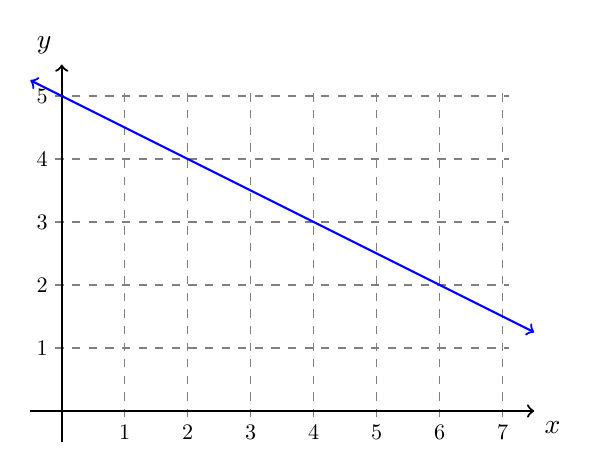
\begin{tikzpicture}[scale=0.8]
\draw[dashed,thin,gray] (-0.1,-0.1) grid (7.1,5.1);
\draw[thick,->] (0,-0.5) -- (0,5.5) node[above left] {$y$};
\draw[thick,->] (-0.5,0) -- (7.5,0) node[below right] {$x$};
\draw[thick,blue,<->] (-0.5,5.25) -- (7.5,1.25) ;
\foreach \x in {1,2,3,4,5,6,7} {
    \draw (\x, -0.1) node[below, scale=0.8] {\x};
}
\foreach \y in {1,2,3,4,5} {
    \draw (-0.1, \y) node[left,scale=0.8] {\y};
}
\end{tikzpicture}
\end{center}

\begin{solution}
\begin{center}
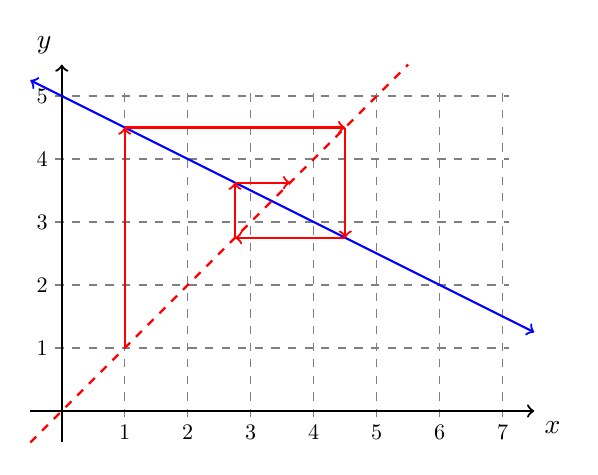
\begin{tikzpicture}[scale=0.8]
\draw[dashed,thin,gray] (-0.1,-0.1) grid (7.1,5.1);
\draw[thick,->] (0,-0.5) -- (0,5.5) node[above left] {$y$};
\draw[thick,->] (-0.5,0) -- (7.5,0) node[below right] {$x$};
\draw[thick,blue,<->] (-0.5,5.25) -- (7.5,1.25) ;
\foreach \x in {1,2,3,4,5,6,7} {
    \draw (\x, -0.1) node[below, scale=0.8] {\x};
}
\foreach \y in {1,2,3,4,5} {
    \draw (-0.1, \y) node[left,scale=0.8] {\y};
}
\draw[dashed,thick, red] (-0.5,-0.5) -- (5.5,5.5);
\draw[->,thick, red] (1,1) -- (1,4.5);
\draw[->,thick, red] (1,4.5) -- (4.5,4.5);
\draw[->,thick, red] (4.5,4.5) -- (4.5,2.75);
\draw[->,thick, red] (4.5,2.75) -- (2.75, 2.75);
\draw[->,thick, red] (2.75,2.75) -- (2.75, 3.625);
\draw[->,thick, red] (2.75, 3.625) -- (3.625, 3.625);
\end{tikzpicture}
\end{center}
\end{solution}

\end{questions}

\end{document}
